%%%%%%%%%%%%%%%%%%%%%%%%%%%%%%%%%%%%%%%%%%%%%%%%%%%%%%%%%%%%%%%%%%%%%%%%%%%%%%%%
%\documentclass[12pt,conference]{ieeeconf} %Github
%\documentclass[letterpaper, 12 pt, onecolumn]{ieeeconf} %Prof. Parallel

% Comment this line out
                                                          % if you need a4paper
\documentclass[a4paper, 12pt, conference]{ieeeconf}      % Use this line for a4
                                                          % paper

\IEEEoverridecommandlockouts                              % This command is only
                                                          % needed if you want to
                                                          % use the \thanks command
\overrideIEEEmargins
% See the \addtolength command later in the file to balance the column lengths
% on the last page of the document

% The following packages can be found on http:\\www.ctan.org
\usepackage{graphics} % for pdf, bitmapped graphics files
\usepackage{epsfig} % for postscript graphics files
%\usepackage{mathptmx} % assumes new font selection scheme installed
%\usepackage{times} % assumes new font selection scheme installed
\usepackage{amsmath} % assumes amsmath package installed
\usepackage{amssymb}  % assumes amsmath package installed

\usepackage{tikz}
\usetikzlibrary{shapes, arrows.meta, positioning}

\usepackage{url}
\usepackage[ruled, vlined, linesnumbered]{algorithm2e}
%\usepackage{algorithm}
\usepackage{verbatim} 
%\usepackage[noend]{algpseudocode}
\usepackage{soul, color}
\usepackage{lmodern}
\usepackage[hidelinks]{hyperref}
\usepackage{fancyhdr}
\usepackage[utf8]{inputenc}
\usepackage{fourier} 
\usepackage{array}
\usepackage{pgf}
\usepackage{makecell}
\usepackage{subcaption}
\usepackage{csvsimple}
\usepackage{pifont}
\usepackage{booktabs}
\usepackage{caption}
\usepackage[normalem]{ulem}
\useunder{\uline}{\ul}{}
\usepackage[sorting=none]{biblatex} % For biblatex
\addbibresource{../reports.bib} % Path to your .bib file

\SetNlSty{large}{}{:}

\renewcommand\theadalign{bc}
\renewcommand\theadfont{\bfseries}
\renewcommand\theadgape{\Gape[4pt]}
\renewcommand\cellgape{\Gape[4pt]}
\newcommand{\cmark}{\ding{51}}
\newcommand{\xmark}{\ding{55}}

\graphicspath{{../../results/rand/dist_plots}{images}}
%\providecommand{\main}{..}
%\graphicspath{{\main/results/rand/dist_plots}}

\newcommand{\rework}[1]{\todo[color=yellow,inline]{#1}}

\makeatletter
\newcommand{\rom}[1]{\romannumeral #1}
\newcommand{\Rom}[1]{\expandafter\@slowromancap\romannumeral #1@}
\makeatother

\pagestyle{plain} 

\title{Comparison of Network Analytics and Significance Analysis on Spotify Artist Feature Collaboration Network\\
\large Learning From Networks - Final report \\}

\author{Fabio Cociancich, Luca Fantin, Alessandro Lincetto % <-this % stops a space 
\\\\ Master Degree in Computer Engineering - University of Padova \\
}

\begin{document}

\maketitle
\thispagestyle{plain}
\pagestyle{plain}

\section{Motivation}

\section{Dataset}

For this project, we used the Spotify Artist Feature Collaboration Network from Kaggle \cite{dataset}. This dataset consists of a graph where nodes correspond to artists and edges connect artists who have collaborated on at least one song. It has 156,422 nodes, which include around 20,000 artists who appeard in the Spotify weekly charts and around 136,000 artists who had at least one feature with the chart artists, and 300,386 edges between them. Out of the information included with the nodes, the ones we used to analyze our results are the following:
\begin{itemize}
    \item artist popularity, expressed as an integer number between 0 and 100 (100 corresponding to the most popular artist on the service), according to the Spotify API;
    \item list of genres, according to the Spotify API.
\end{itemize}

\section{Measures} \label{sec:measures}

The measures considered for these analyses are both graph- and node-level graph metrics. At the graph level, we compute the number of connected components and the clustering coefficient of the graph, both global and average. At the node level, instead, we have the local clustering coefficients and a series of centrality measures. Alongside those presented during the lectures (degree, closeness, betweenness, PageRank), we also considered the \emph{eigenvector centrality}, which is built on the intuition that a node is important if it is connected to other important nodes. Given a graph $G=(V,E)$, let us define $\textbf{x}\in\mathbb{R}^{|V|}$ the vector of the centrality values for all nodes in $G$, $A$ the adjacency matrix of $G$ and $\lambda\neq 0$ a constant. For any node $i$ we can write: $$x_i=\frac{1}{\lambda}\sum_{j=1}^{|V|}A_{i,j}x_j \quad \rightarrow \quad Ax=\lambda x$$
The mathematical representation of the intuition can thus be reformulated as finding the eigenvector of the adjacency matrix corresponding to the eigenvalue $\lambda$; such vector includes the values of the eigenvector centrality for all nodes. This centrality measure has been studied extensively \cite{Bonacich2007} \cite{Borgatti2006} \cite{Spizzirri2011}, also in the context of social media network analysis \cite{Maharani2014}, including Spotify \cite{South2021} \cite{South2018}.  

\section{Significance analysis framework}

The significance analysis we performed is composed by the statistical testing framework and the random graph model chosen. For the latter, we chose the \emph{Holme-Kim model} \cite{Holme2002}. The generation of a random graph starts from a number of nodes smaller than the desired graph size and no edges, iteratively adds new nodes and connects them with already existing ones with a distribution that favours nodes with an already high degree. The resulting graphs show a power-law distribution of the degrees: the probability of seeing a node with a certain degree decreases exponentially as the degree increases. Such characteristic is observed in many real-world networks and is captured by this model more accurately compared to the Erd\H{o}s-R\'{e}nyi model. Furthermore, this model produces graphs with tunable global clustering coefficients by creating additional edges: once a newly created node $v$ is connected to an existing one $w$, a new edge is created between $v$ and one of the neighbours of $w$ with a certain probability.

The null hypothesis considered in this project states that the metric values computed on the real graph well conform to the distribution determined by the generated random graphs, which implies our Spotify dataset does not have any significant feature that can explain the values we compute. Our statistical testing procedures consists of two steps. Any statistical test assumes that the considered population has a known distribution, most often a Gaussian one. Because of the specificity of our random graph model, the first step computes how similar the distribution of the metric we are considering is compared to a Gaussian distribution, through a \emph{normality test}. We used Shapiro-Wilk test \cite{ShapiroWilk1965}, since it is considered the most powerful normality test available \cite{RazaliYap2011}. The second step then checks the validity of our null hypothesis by computing the probability that the random distribution of the metric generates a value greater or lower than the real value, also called p-value.

\section{Code}

All the code developed for this project, together with results files, dataset files and more, can be found in our GitHub repository \cite{githubRepo}. The central script is \texttt{main.py}, which computes any combination of the measures presented in section \ref{sec:measures} on various graphs, depending on the command line arguments provided. The script can work on the entire dataset, subgraphs taken from the dataset with respect to certain genres or popularity thresholds, and random graphs generated with the Holme-Kim model \cite{Holme2002} with parameters specified through the command line arguments. The libraries NetworkX and NetworKit are used to represent the graphs \cite{NetworkX_Graph}, compute the metrics \cite{NetworkX_Centrality} \cite{NetworKit_local_clustering} \cite{NetworKit_globals_clustering} and generate the random graphs \cite{NetworkX_HolmeKim}.

\section{Experimental setup}

All computations on graphs have been performed on the CAPRI High-Performance Computing (HPC) cluster \cite{capri}. The hardware capabilities and the presence of the SLURM job scheduler system allowed us to perform heavy computations in a feasible time frame. This system features the following hardware:
\begin{itemize}
    \item 16 Intel(R) Xeon(R) Gold 6130 @ 2.10GHz CPUs
    \item 6 TB DDR4 RAM
    \item 2 NVIDIA Tesla P100 16GB GPUs
    \item 40 TB of disk space
\end{itemize}

On the other side, the analysis of the data computed by the cluster has been performed on our local machines. They all employ AMD Ryzen 5/7 CPUs and RAMs ranging from 8 GBs and 24 GBs.

\section{Data analysis on whole dataset}
In the first part of the analysis, artist rankings were calculated and sorted based on two key centrality metrics: degree centrality and closeness centrality. Degree centrality identified artists with the highest number of direct connections (i.e., those who collaborate with the most artists), so these artists occupy the top positions in the ranking. Some of the top-ranked artists include Johann Sebastian Bach, Traditional, Mc Gw, MC MN, and Jean Sibelius, who stand out for their high number of collaborations. Closeness centrality, on the other hand, highlighted artists who are more "central" in the network, meaning those who, despite having fewer direct collaborations, are well-positioned to interact with the entire network. Artists such as R3HAB, Snoop Dogg, Diplo, David Guetta, and Tiësto are at the top of this ranking, indicating their global influence within the network.

We have created a visual representation of the distribution of centrality measures for each artist. The resulting graph clearly shows how some measures, such as degree centrality, are widely distributed, with many nodes having a low number of collaborations and a few nodes having a very high number. Closeness centrality, on the other hand, tends to concentrate within a narrow range, suggesting that many artists are relatively close in the network, while some are significantly distant from the rest of the graph. Betweenness, PageRank, and eigenvector centrality show a similar distribution, with many nodes having low values and a few emerging with higher values, indicating that there are artists with very high influence in the network, but they are few. The comparison among the different centrality measures highlights how each of them measures different aspects of the structure and dynamics of the network.

Following this, the average ranking for each artist was calculated, based on the combination of rankings obtained through the various centrality metrics (degree, closeness, betweenness, PageRank, eigenvector centrality). This average ranking provided an overall view of the importance of each artist within the network, taking into account all dimensions of centrality. Artists like Snoop Dogg, Gucci Mane, and David Guetta emerged as the most important based on this average ranking, consistently ranking high across various metrics.

A complete ranking of the artists was finally calculated, based on all the centrality measures analyzed: degree, closeness, betweenness, PageRank, eigenvector centrality, and an average ranking that integrates the results of all the metrics. Betweenness centrality identifies artists who act as "bridges" between different areas of the network, such as Snoop Dogg, Gucci Mane, and David Guetta, while PageRank and eigenvector centrality highlight artists connected to important nodes, boosting their centrality value. The average ranking provides a comprehensive summary of the artists' importance, combining all the metrics. The analysis shows that some artists, such as Snoop Dogg and David Guetta, rank high in multiple rankings, suggesting their central and influential role in the collaboration network.

\section{Data analysis on subgraphs}
\section{Data analysis on subgraphs}
The analysis of subgraphs about genres reveals that there are significant variability among various types of music. 
Betweenness shows a non-uniform distribution; some genres have concentrated values, suggesting a more homogeneous "bridge" role, while others are more dispersed. 
Similarly, closeness does not exhibit a uniform distribution, with some genres being closer to each other and others more distant, indicating heterogeneity in proximity between genres. 
The clustering coefficient generally shows high values, but with a wide distribution, highlighting that while there is a tendency to form clusters, it is not uniform. The degree presents a heterogeneous distribution: some genres have more connections, while others have fewer. 
The eigenvector shows a variable distribution, with some genres more concentrated at specific values. PageRank, on the other hand, displays a more concentrated distribution, with values less dispersed compared to the other metrics. 
The correlation matrix reveals that some metrics, such as betweenness, degree, PageRank, and eigenvector, are strongly correlated with each other, while the clustering coefficient appears less correlated, suggesting that the tendency to form clusters depends on distinct factors.
In the end we have considered the most popular artists in a subgraph and we can notice that the general metrics are higher than the real graph.


\section{Data analysis on random graphs}

For the significance analysis we considered the real graph and a selection of subgraphs. Because of the NetworkX implementation of the Holme-Kim, these graphs had to have more edges than nodes and a global clustering coefficient lower than 0.3 to be accurately resembled by the random graphs. For each of these graphs, 200 random graphs were generated, with the same number of nodes, a similar number of edges and a comparable global clustering coefficient. The last part was easy for graphs with a coefficient under 0.1, but reaching values above that threshold became almost impossible. On these generated graphs, we computed all available graph-level metrics and the maximum and average value of the closeness and eigenvector centralities, in order to represent both distributions of the node rankings with respect to centrality values. The closeness centrality was not computed for the larger graphs, corresponding to the entire dataset and the pop genre subgraph, due to time constraints.

\subsection{Normality test}

For each set of random graphs generated, all values of the metrics were tested against a Gaussian distribution using the Shapiro-Wilk test. The result, reported in table \ref{tab:normality}, was that most of the distributions could be assimilated to a Gaussian one. For the other ones, plotting the histogram of the values revealed a distribution graphically resembling a Gaussian curve. Thus, we decided to take into consideration all metrics for all sets of graphs for the next phase of statistical testing.

\subsection{p-value computation}

For each metric listed in this section, we took its value from the real (sub)graph and computed the probabilities that the Gaussian distribution corresponding to the random graphs give a value higher or lower than the real one. The results, reported in table \ref{tab:pvalue}, show that we cannot accept our null hypothesis, thus we can say that our (sub)graphs have particular features that affect the metric values in some significant way. In fact, for almost all graphs, if the real ones were generated by the same distribution as the random graphs, we should expect to see higher maximum and average values for the considered centralities, a higher average clustering coefficient and a lower global clustering coefficient. The latter results confirms the difficulties in replicating the value computed on the real graphs through the random graph model. The results for the other metrics could be due to the more fragmented nature of the real graph, which has a large number of connected components and less edges.

\section{Future work}

Our analysis on the whole dataset and its genre subgraphs is mainly concerned with the node-level metrics. Future extensions of our work could be comparing the graph-level metrics of these graphs to study how network dynamic change within the whole network between different genres.

Another open field is using the other features included in the dataset, like the number of followers and the number of chart hits of each artist, for the same analyses presented in this report. This also includes using the popularity level more extensively than what has been reported here.

\section{Contributions}

Out of the work presented in this report, Luca Fantin wrote the code for the random graphs 
and for the analysis of such and the refactoring of the code.
Fabio Cociancich wrote the scripts to create subgraphs based on genre, artists, 
popularity threshold and given  x\% top popular artists, the scripts to 
compute the metrics of a graph, he analyzed them and saved the results in the csv files.
Alessandro Lincetto wrote scripts for generating random graphs with powerlaw\_cluster,
he generated some csv files, the scripts to create graphs from the csv files and 
the initial code for the metrics of graphs.
Each member wrote the report section related to their work.
The percentage of work done can thus be estimated to be 40\%, 30\%, 30\% respectively.



\newpage
  
% Please add the following required packages to your document preamble:
% \usepackage[normalem]{ulem}
% \useunder{\uline}{\ul}{}

\begin{table*}[]
    \begin{tabular}{|c|c|c|c|c|c|c|c|c|c|c|}
    \hline
    \textbf{\#}           & \textit{\textbf{1}}                                        & \textit{\textbf{2}}                                         & \textit{\textbf{3}}                                           & \textit{\textbf{4}}                                         & \textit{\textbf{5}}                                    & \textit{\textbf{6}}                                             & \textit{\textbf{7}}                                      & \textit{\textbf{8}}                                     & \textit{\textbf{9}}                                    & \textit{\textbf{10}}                                      \\ \hline
    \textit{Degree}       & Johann Sebastian Bach                                      & Traditional                                                 & Mc Gw                                                         & MC MN                                                       & Jean Sibelius                                          & Armin van Buuren                                                & Gucci Mane                                               & Steve Aoki                                              & Snoop Dogg                                             & Diplo                                                     \\ \hline
    \textit{Closeness}    & R3HAB                                                      & Snoop Dogg                                                  & Diplo                                                         & David Guetta                                                & Tiësto                                                 & Steve Aoki                                                      & Major Lazer                                              & Pitbull                                                 & Sean Paul                                              & French Montana                                            \\ \hline
    \textit{Betweenness}  & Snoop Dogg                                                 & Traditional                                                 & R3HAB                                                         & Diplo                                                       & Johann Sebastian Bach                                  & Tiësto                                                          & Major Lazer                                              & Steve Aoki                                              & Pitbull                                                & David Guetta                                              \\ \hline
    \textit{PageRank}     & Johann Sebastian Bach                                      & Traditional                                                 & Jean Sibelius                                                 & Mc Gw                                                       & MC MN                                                  & HaKokhav HaBa                                                       & John Williams                                            & A.R. Rahman                                             & Armin van Buuren                                       & Snoop Dogg                                                \\ \hline
    \textit{Eigenvector}  & Farruko                                                    & French Montana                                              & Gucci Mane                                                    & Ty Dolla \$ign                                              & Lil Wayne                                              & Chris Brown                                                     & Snoop Dogg                                               & De La Ghetto                                            & J Balvin                                               & Future                                                    \\ \hline
    \textit{Average rank} & \begin{tabular}[c]{@{}c@{}}Snoop Dogg\\ (5.8)\end{tabular} & \begin{tabular}[c]{@{}c@{}}Gucci Mane\\ (11.6)\end{tabular} & \begin{tabular}[c]{@{}c@{}}David Guetta\\ (18.8)\end{tabular} & \begin{tabular}[c]{@{}c@{}}Steve Aoki\\ (19.0)\end{tabular} & \begin{tabular}[c]{@{}c@{}}Diplo\\ (20.8)\end{tabular} & \begin{tabular}[c]{@{}c@{}}French Montana\\ (21.0)\end{tabular} & \begin{tabular}[c]{@{}c@{}}Pitbull\\ (23.4)\end{tabular} & \begin{tabular}[c]{@{}c@{}}Tiesto\\ (23.6)\end{tabular} & \begin{tabular}[c]{@{}c@{}}R3HAB\\ (24.4)\end{tabular} & \begin{tabular}[c]{@{}c@{}}The Game\\ (27.0)\end{tabular} \\ \hline
    \end{tabular}
    \caption{Top 10 artists in the whole dataset, according to our centrality measures. The "average rank" row also reports the value for each artist.}
    \label{tab:ranking}
    \end{table*}

\begin{table*}[]
    \centering
    \begin{tabular}{|c|c|c|c|c|c|c|c|}
    \hline
    \textbf{Reference graph}                                                       & \textit{Average cc} & \textit{Global cc} & \textit{\begin{tabular}[c]{@{}c@{}}Approximate\\ global cc\end{tabular}} & \textit{\begin{tabular}[c]{@{}c@{}}Maximum\\ eigenvector\end{tabular}} & \textit{\begin{tabular}[c]{@{}c@{}}Average\\ eigenvector\end{tabular}} & \textit{\begin{tabular}[c]{@{}c@{}}Maximum\\ closeness\end{tabular}} & \textit{\begin{tabular}[c]{@{}c@{}}Average\\ closeness\end{tabular}} \\ \hline
    \textbf{House subgraph}                                                        & \xmark              & \cmark             & \cmark                                                                   & \cmark                                                                 & \cmark                                                                 & \cmark                                                               & \cmark                                                               \\ \hline
    \textbf{Pop subgraph}                                                          & \xmark              & \xmark             & \xmark                                                                   & \cmark                                                                 & \cmark                                                                 &                                                                      &                                                                      \\ \hline
    \textbf{Rap subgraph}                                                          & \xmark              & \xmark             & \xmark                                                                   & \cmark                                                                 & \cmark                                                                 & \cmark                                                               & \xmark                                                               \\ \hline
    \textbf{Whole dataset}                                                         & \xmark              & \xmark             & \xmark                                                                   & \cmark                                                                 & \cmark                                                                 &                                                                      &                                                                      \\ \hline
    \textbf{\begin{tabular}[c]{@{}c@{}}Top 10\%\\ popularity subgraph\end{tabular}} & \xmark              & \xmark             & \xmark                                                                   & \cmark                                                                 & \cmark                                                                 & \xmark                                                               & \xmark                                                               \\ \hline
    \textbf{Trap subgraph}                                                         & \xmark              & \xmark             & \xmark                                                                   & \cmark                                                                 & \cmark                                                                 & \cmark                                                               & \xmark                                                               \\ \hline
    \end{tabular}
    \caption{Results of the Shapiro-Wilk normality tests for all considered graphs. The "reference graph" is the graph to which the random graphs used in the analysis refer to. "cc" stands for "clustering coefficient".}
    \label{tab:normality}
\end{table*}

\begin{table*}[]
  \centering
  \begin{tabular}{|c|c|c|c|c|c|c|c|}
  \hline
  \textbf{Reference graph}                                                        & \textit{Average cc}     & \textit{Global cc}   & \textit{\begin{tabular}[c]{@{}c@{}}Approximate\\ global cc\end{tabular}} & \textit{\begin{tabular}[c]{@{}c@{}}Maximum\\ eigenvector\end{tabular}} & \textit{\begin{tabular}[c]{@{}c@{}}Average\\ eigenvector\end{tabular}} & \textit{\begin{tabular}[c]{@{}c@{}}Maximum\\ closeness\end{tabular}} & \textit{\begin{tabular}[c]{@{}c@{}}Average\\ closeness\end{tabular}} \\ \hline
  \textbf{House subgraph}                                                         & \textbf{\textgreater{}} & \textbf{\textless{}} & \textbf{\textless{}}                                                     & \textbf{\textgreater{}}                                                & \textbf{\textgreater{}}                                                & \textbf{\textgreater{}}                                              & \textbf{\textgreater{}}                                              \\ \hline
  \textbf{Pop subgraph}                                                           & \textbf{\textgreater{}} & \textbf{\textless{}} & \textbf{\textless{}}                                                     & \textbf{\textgreater{}}                                                & \textbf{\textgreater{}}                                                & \textbf{}                                                            & \textbf{}                                                            \\ \hline
  \textbf{Rap subgraph}                                                           & \textbf{\textgreater{}} & \textbf{\textless{}} & \textbf{\textless{}}                                                     & \textbf{\textgreater{}}                                                & \textbf{\textgreater{}}                                                & \textbf{\textgreater{}}                                              & \textbf{\textgreater{}}                                              \\ \hline
  \textbf{Whole dataset}                                                          & \textbf{\textgreater{}} & \textbf{\textless{}} & \textbf{\textless{}}                                                     & \textbf{\textgreater{}}                                                & \textbf{\textless{}}                                                   & \textbf{}                                                            & \textbf{}                                                            \\ \hline
  \textbf{\begin{tabular}[c]{@{}c@{}}Top 10\%\\ popularity subgraph\end{tabular}} & \textbf{\textgreater{}} & \textbf{\textless{}} & \textbf{\textless{}}                                                     & \textbf{\textgreater{}}                                                & \textbf{\textgreater{}}                                                & \textbf{\textgreater{}}                                              & \textbf{\textgreater{}}                                              \\ \hline
  \textbf{Trap subgraph}                                                          & \textbf{\textgreater{}} & \textbf{\textless{}} & \textbf{\textless{}}                                                     & \textbf{\textgreater{}}                                                & \textbf{\textgreater{}}                                                & \textbf{\textgreater{}}                                              & \textbf{\textgreater{}}                                              \\ \hline
  \end{tabular}
  \caption{Results of the p-value computations: the contents of the cells represent how we should expect the metric values to be, compared to the values computed on the real (sub)graphs, if we were to accept our null hypothesis. "cc" stands for "clustering coefficient".}
  \label{tab:pvalue}
\end{table*}

\begin{figure*}
    \centering
    \begin{subfigure}{.33\textwidth}
      \centering
      \captionsetup{justification=centering}
      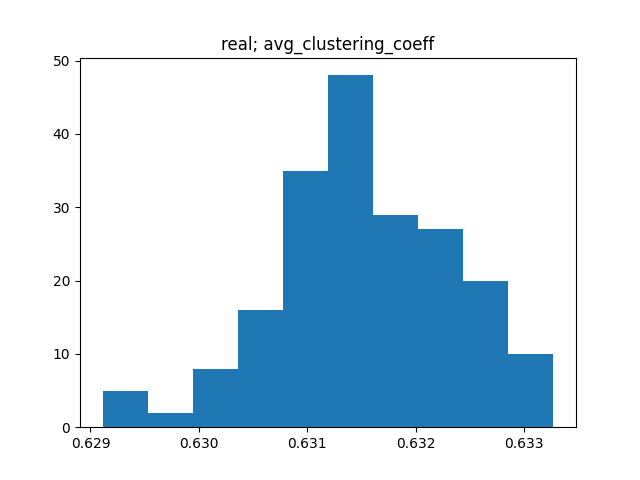
\includegraphics[width=\linewidth]{dist_plot_real_avg_clustering_coeff.png}
      \caption{Whole dataset, average \\ clustering coefficient}
      \label{fig:hist1}
    \end{subfigure}%
    \begin{subfigure}{.33\textwidth}
      \centering
      \captionsetup{justification=centering}
      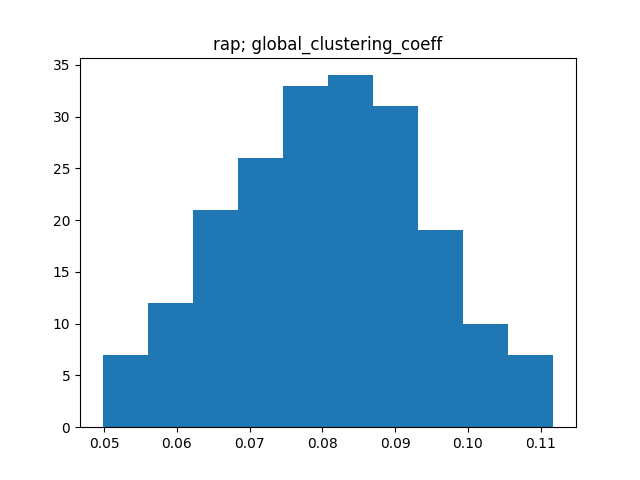
\includegraphics[width=\linewidth]{dist_plot_rap_global_clustering_coeff.png}
      \caption{Rap subgraph, global \\ clustering coefficient}
      \label{fig:hist2}
    \end{subfigure}
    \begin{subfigure}{.33\textwidth}
      \centering
      \captionsetup{justification=centering}
      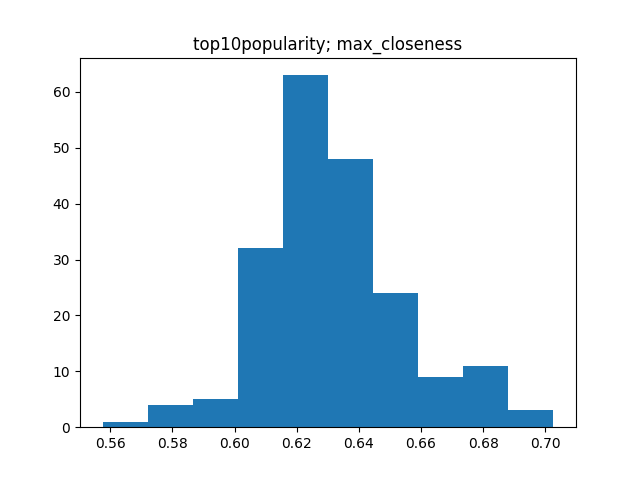
\includegraphics[width=\linewidth]{dist_plot_top10popularity_max_closeness.png}
      \caption{Top 10\% popularity subgraph, maximum closeness}
      \label{fig:hist3}
    \end{subfigure}
    \begin{subfigure}{.33\textwidth}
      \centering
      \captionsetup{justification=centering}
      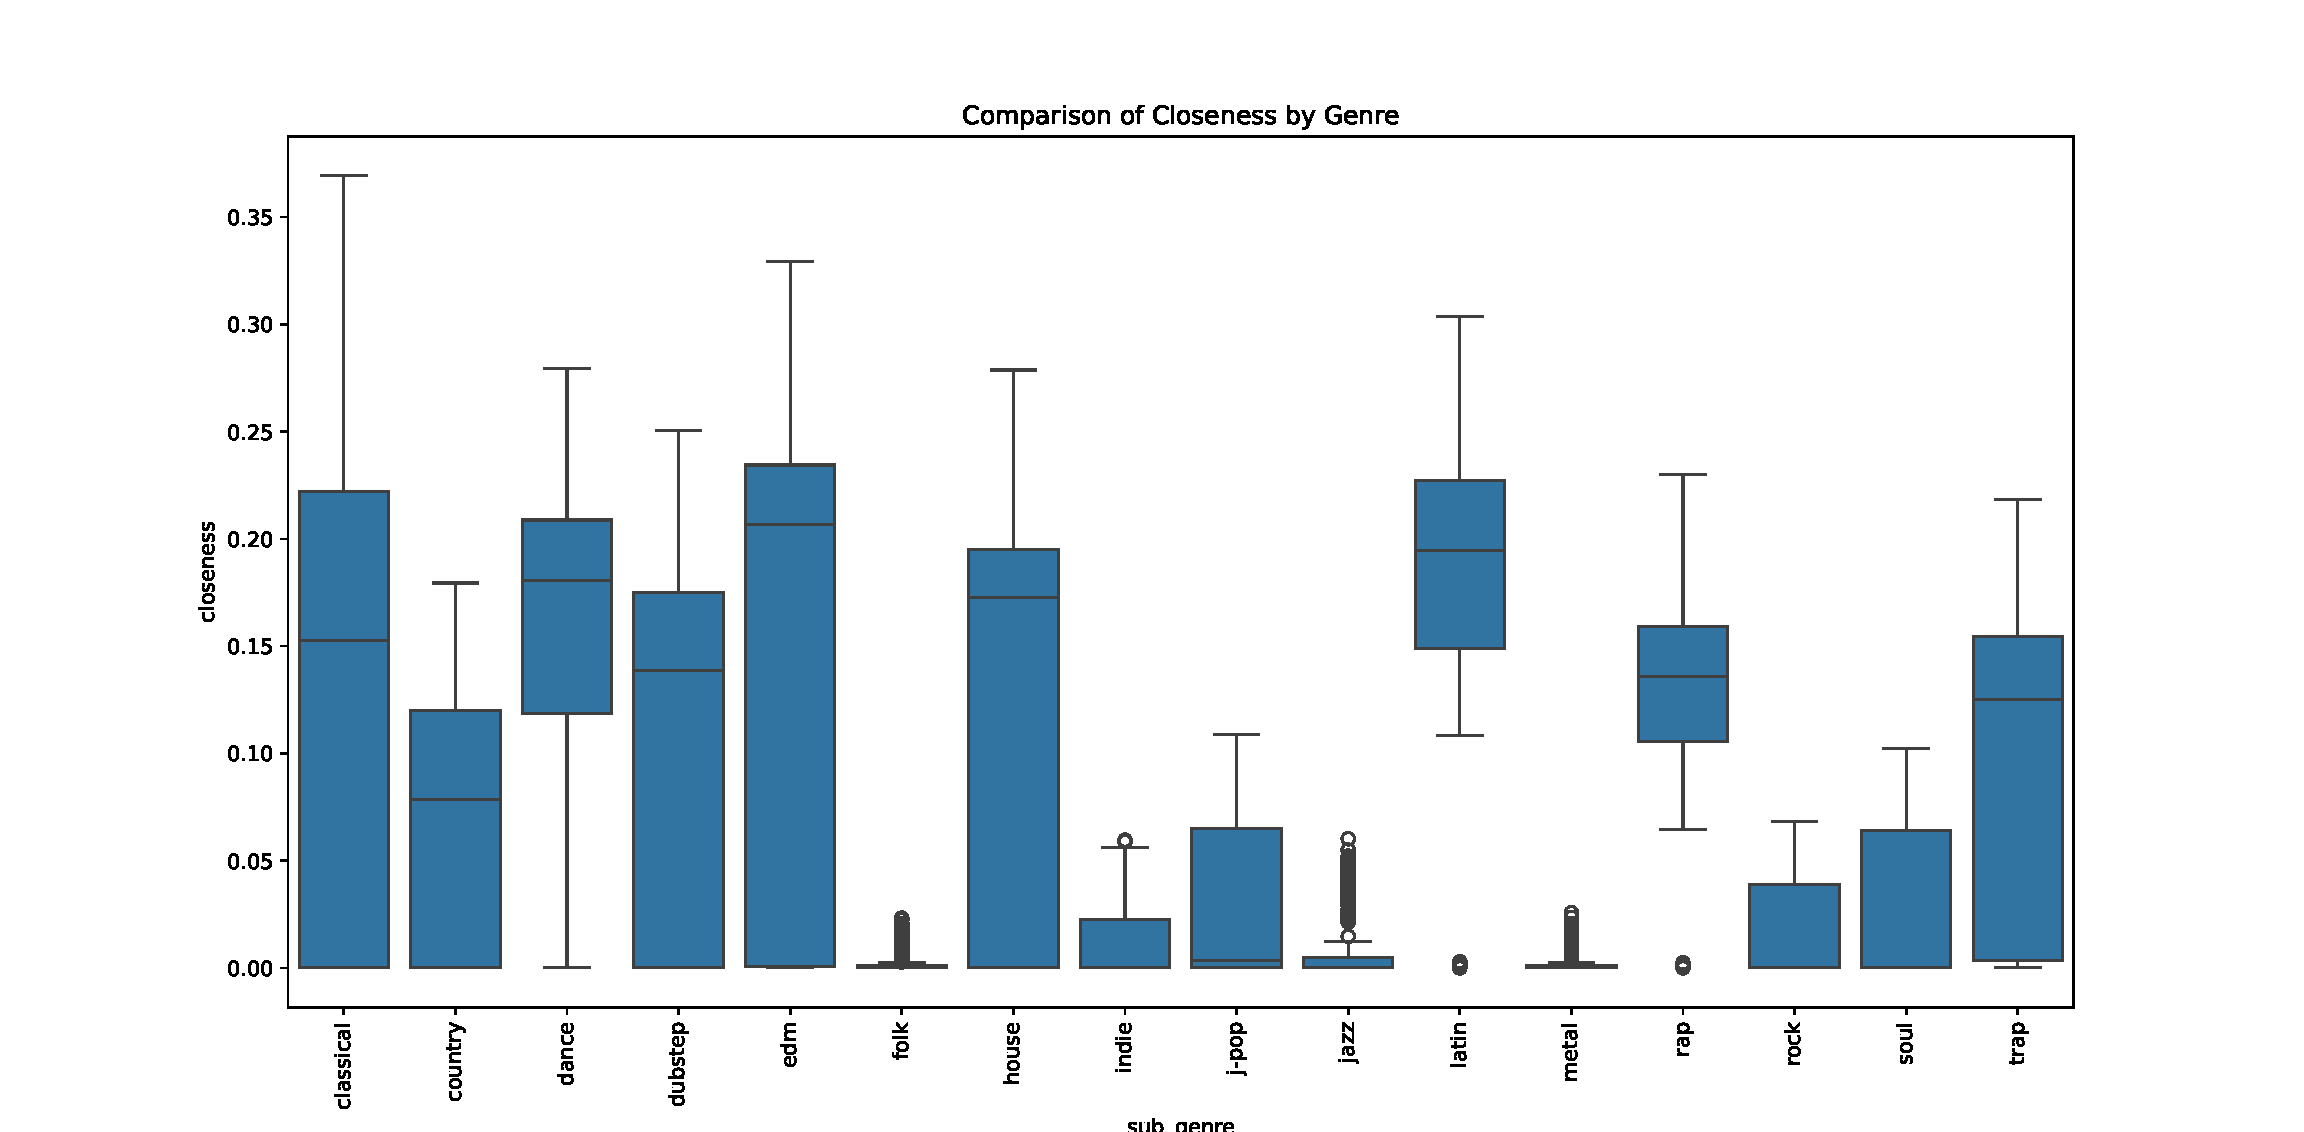
\includegraphics[width=\linewidth]{../../results/sub_genre/closeness.pdf}  % Usa \includegraphics per il PDF
      \caption{closeness plot}
      \label{fig:hist4}
    \end{subfigure}
    \begin{subfigure}{.33\textwidth}
      \centering
      \captionsetup{justification=centering}
      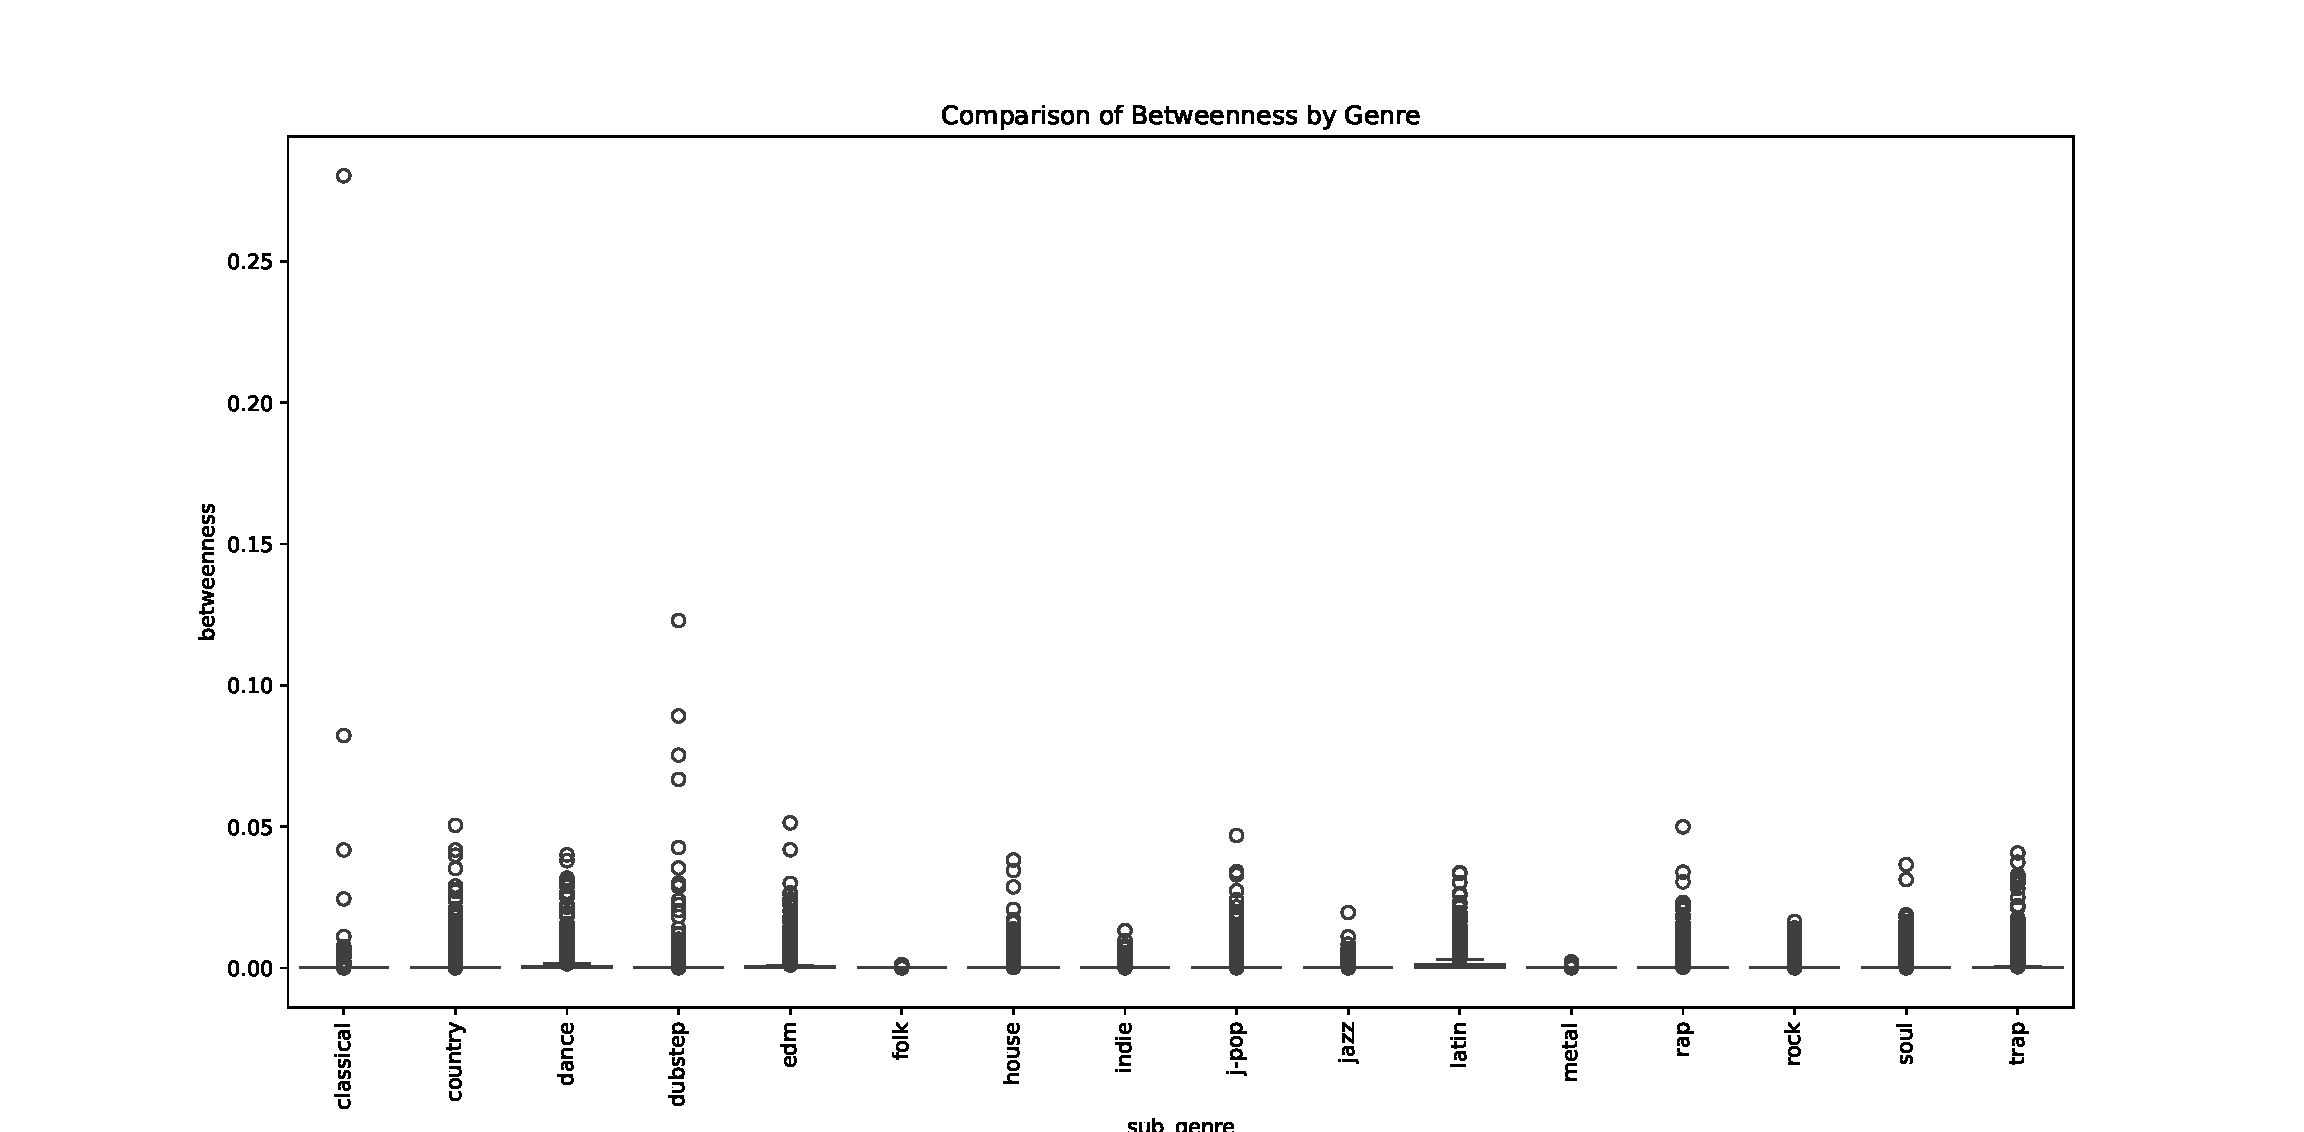
\includegraphics[width=\linewidth]{../../results/sub_genre/betweenness.pdf}  % Usa \includegraphics per il PDF
      \caption{betweenness plot}
      \label{fig:hist5}
    \end{subfigure}
    \begin{subfigure}{.33\textwidth}
      \centering
      \captionsetup{justification=centering}
      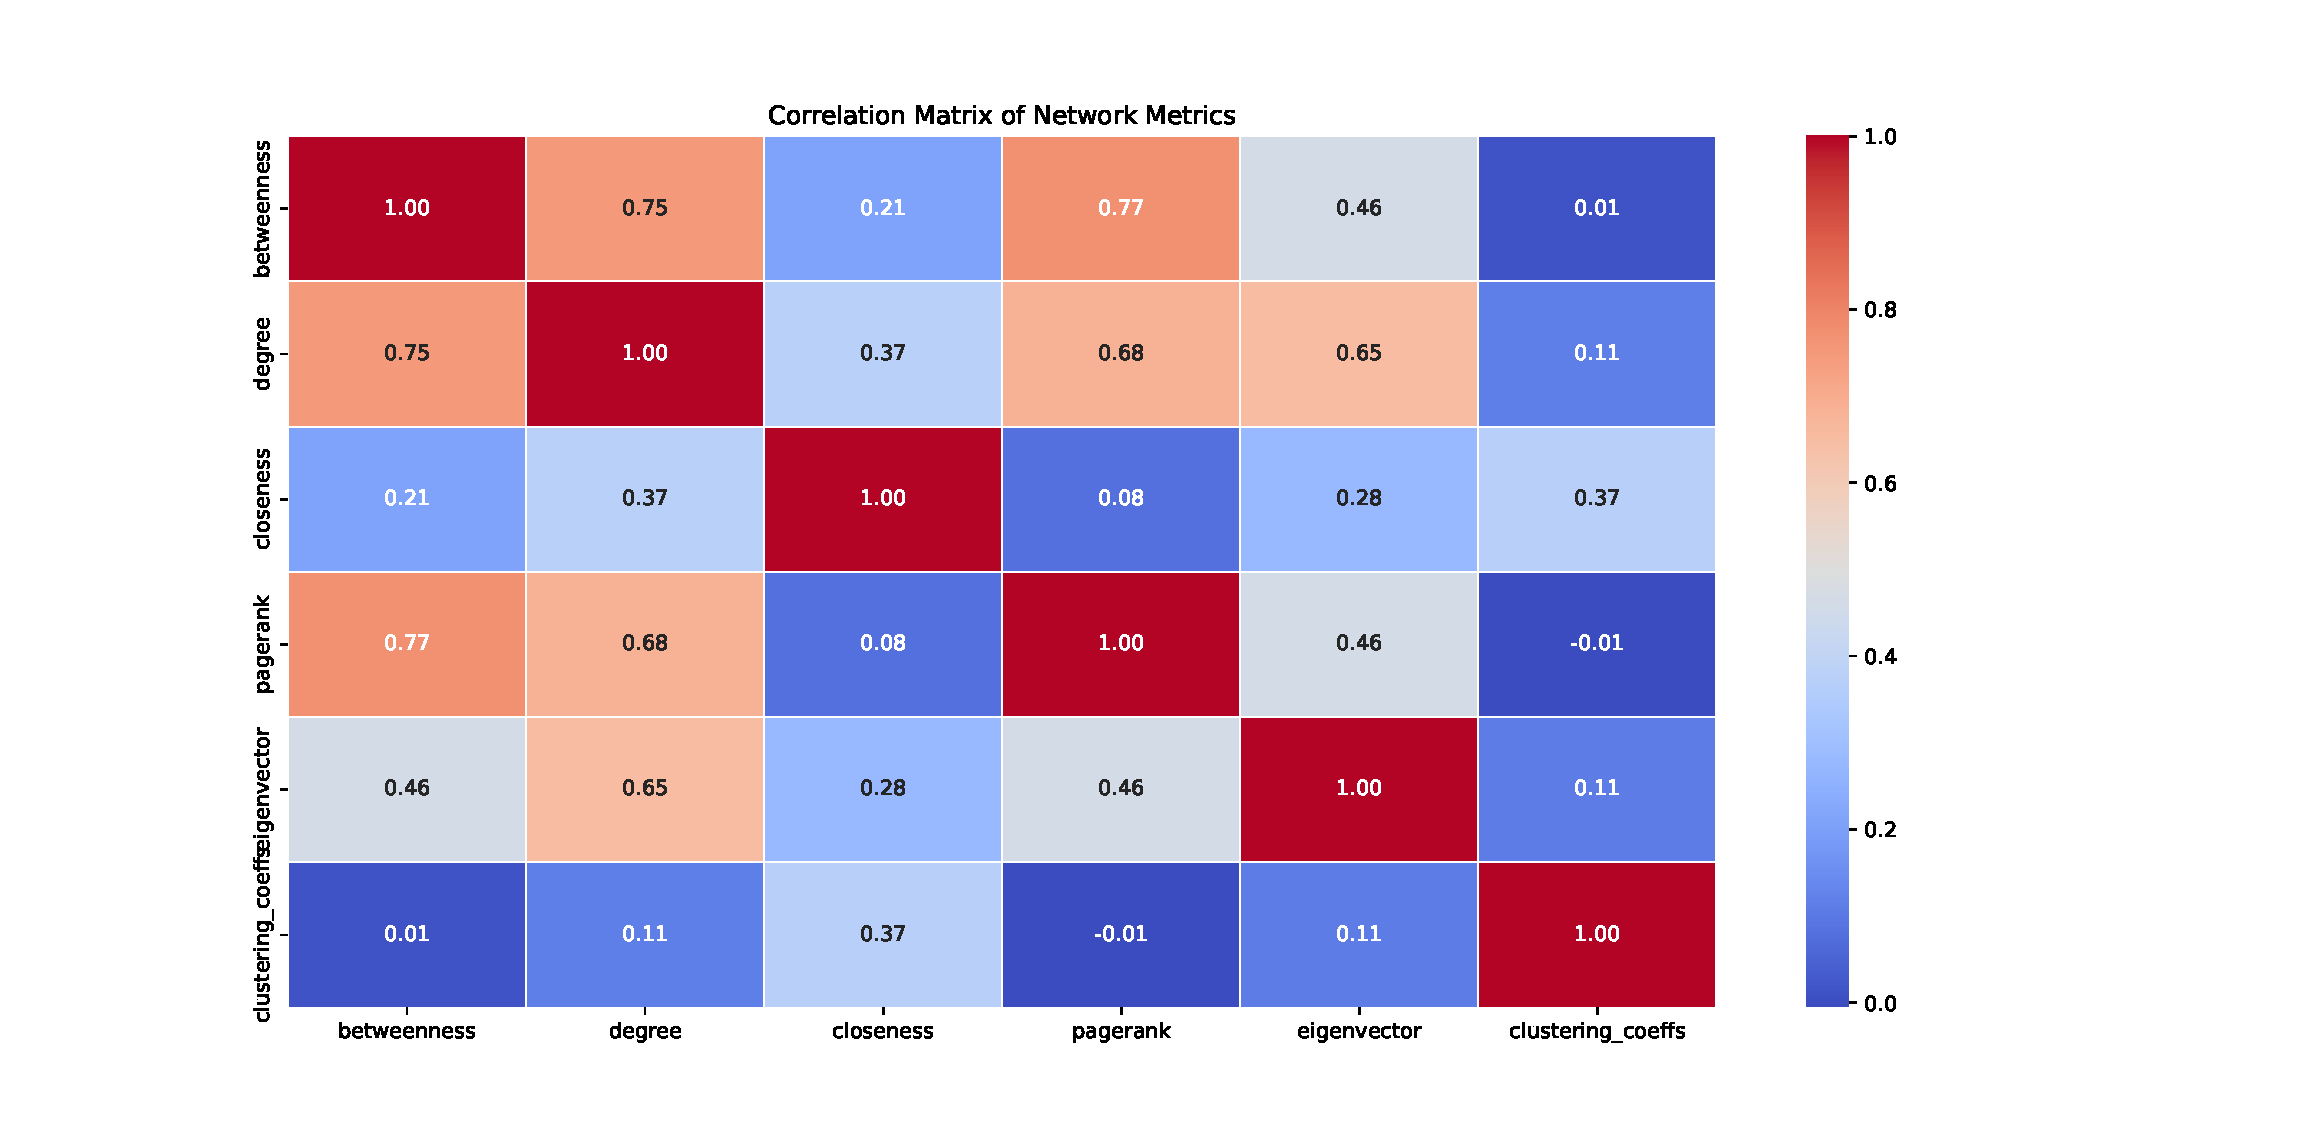
\includegraphics[width=1.25\linewidth, height=3cm]{../../results/sub_genre/correlation_matrix.pdf}  % Usa \includegraphics per il PDF
      \caption{Correlation Matrix}
      \label{fig:hist6}
    \end{subfigure}
    \caption{Example of histograms for the metrics computed on random graphs that do not have a Gaussian distribution according to the Shapiro-Wilk test.}
    \label{fig:hist}
\end{figure*}

\clearpage

\printbibliography[nottype=online]
\end{document}
